\newpage
\def\thoigian{90}%--Thời gian
\de{Đề số 2}{Chương II. Vectơ và hệ tọa độ trong không gian}


\begin{center}
	\textbf{PHẦN 1 - Câu trắc nghiệm nhiều phương án lựa chọn.}
\end{center}
\setcounter{ex}{0}
\Opensolutionfile{ans}[ans-ABCD]

\begin{ex}%[2H2N1-2]
	\immini[thm]{Cho hình hộp $ABCD.A’B’C’D’$.
		Khi đó, $\overrightarrow{AA’}+\overrightarrow{AD}$ bằng
		\choice
		{\True $\overrightarrow{AD’}$}
		{$\overrightarrow{AB’}$}
		{$\overrightarrow{AC’}$}
		{$\overrightarrow{AC}$}
	}{\begin{tikzpicture}[scale=0.6, font=\footnotesize, line join=round, line cap=round, >=stealth]
			\def\a{3.5}
			\def\h{4}
			\path (0:0) coordinate (A)
			++(0:\a) coordinate (D)
			++(-130:\a/2) coordinate (C)
			($(A)+(C)-(D)$) coordinate (B)
			($(A)!0.25!(C)$) coordinate (H)
			($(H)+(90:\h)$) coordinate (A')
			($(A')+(C)-(A)$) coordinate (C')
			($(C')+(B)-(C)$) coordinate (B')
			($(A')+(D)-(A)$) coordinate (D');
			\draw[dashed] (B)--(A)--(A') (A)--(D);
			\draw (C)--(C') (D)--(D') (B)--(B') (B)--(C)--(D) (A')--(B')--(C')--(D')--cycle;
			\foreach \x/\g in {A/180,B/180,C/0,D/0,A'/180,B'/180,C'/0,D'/0}
			\fill (\x) circle (1pt)
			($(\g:4mm)+(\x)$) node {$\x$};
		\end{tikzpicture}
	}
	\loigiai{
		Theo quy tắc hình bình hành, ta có $\overrightarrow{AA’}+\overrightarrow{AD}=\overrightarrow{AD’}$.
	}
\end{ex}

\begin{ex}%[2H2N1-3]
	\immini[thm]{
		Cho hình hộp chữ nhật $A BCD.A'B'C' D'$. Mệnh đề nào sau đây đúng?	
		\choice[2]
		{$\overrightarrow{AB} \cdot \overrightarrow{BA'}=0$}
		{\True $\overrightarrow{AB} \cdot \overrightarrow{BB'}=0$}
		{$\overrightarrow{AB} \cdot \overrightarrow{AB'}=0$}
		{$\overrightarrow{AB} \cdot \overrightarrow{A'B'}=0$}
	}{
		\begin{tikzpicture}[scale=0.7,font=\footnotesize,line join=round,line cap=round,>=stealth]
			\path
			(0,0) coordinate (B)
			(1,0.8) coordinate (A)
			(4,0) coordinate (C)
			($(C)-(B)+(A)$) coordinate (D)	
			($(A)+(90:3.5)$) coordinate (A')
			($(B)-(A)+(A')$) coordinate (B')
			($(C)-(A)+(A')$) coordinate (C')
			($(D)-(A)+(A')$) coordinate (D')
			;
			\draw (B')--(B)--(C)--(D)--(D')--(A')--(B')--(C')--(D') (C)--(C');
			\draw[dashed] (A)--(D) (A')--(A)--(B);
			\foreach \p/\q in {A/160,B/-135,C/-45,D/0,A'/90,B'/180,C'/-20,D'/0}
			\fill[black] (\p)node[shift={(\q:3mm)}]{$\p$} circle (1.0pt);	
		\end{tikzpicture}
	}
	\loigiai{
		Ta có $AB \perp BB' \Rightarrow \overrightarrow{AB} \cdot \overrightarrow{BB'}=0$.}
\end{ex}
\begin{ex}%[2H2N1-3]
	Cho $\overrightarrow{a}$ và $\overrightarrow{b}$ là hai vectơ ngược hướng và đều khác vectơ $\overrightarrow{0}$. Mệnh đề nào sau đây đúng?
	\choice
	{$\overrightarrow{a} \cdot \overrightarrow{b}=\left| \overrightarrow{a}\right| \cdot \left| \overrightarrow{b}\right|$}
	{$\overrightarrow{a} \cdot \overrightarrow{b}=0$}
	{$\overrightarrow{a} \cdot \overrightarrow{b}=-1$}
	{\True $\overrightarrow{a} \cdot \overrightarrow{b}=-\left| \overrightarrow{a}\right| \cdot \left| \overrightarrow{b}\right|$}
	\loigiai{
		Do $\overrightarrow{a}$ và $\overrightarrow{b}$ là hai vectơ ngược hướng và đều khác vectơ $\overrightarrow{0}$ nên $\left( \overrightarrow{a}, \overrightarrow{b}\right) =180^{\circ} $.\\
		Suy ra $\overrightarrow{a} \cdot \overrightarrow{b}=-\left| \overrightarrow{a}\right| \cdot \left| \overrightarrow{b}\right|$.
	}
\end{ex}


\begin{ex}%[2H2N2-3]
	Trong không gian $Oxyz$, cho hai điểm $A(-1;1;-2)$, $B(1;3;0)$. Khi đó
	\choice
	{$\overrightarrow{AB}=(-2;-2;-2)$}
	{$\overrightarrow{AB}=(0;2;-1)$}
	{\True $\overrightarrow{AB}=(2;2;2)$}
	{$\overrightarrow{AB}=(0;4;-2)$}
	\loigiai{
		Ta có $\overrightarrow{AB}=(2;2;2)$.
	}
\end{ex}


\begin{ex}%[2H2H2-2]
	Trong không gian $Oxyz$, cho các điểm $A(2;1;-1)$, $B(2;-2;-1)$. Tọa độ của điểm $M$ thỏa mãn hệ thức $\overrightarrow{MA}+2\overrightarrow{MB}=\overrightarrow{0}$ là
	\choice
	{$(-2;-1;2)$}
	{\True $(2;-1;-1)$}
	{$(1;3;1)$}
	{$(-1;-3;-1)$}
	\loigiai{
		$\overrightarrow{MA}=(2-x;1-y;-1-z), \quad \overrightarrow{MB}=(2-x;-2-y;-1-z)$.\\
		Ta có
		$\overrightarrow{MA}+2\overrightarrow{MB}=\overrightarrow{0} \Leftrightarrow \heva{&2-x+2(2-x)=0\\&1-y+2(-2-y)=0\\&-1-z+2(-1-z)=0}
		\Leftrightarrow
		\heva{&x=2\\&y=-1\\&z=-1}$.
		Vậy $M(2;-1;-1)$.
	}
\end{ex}

\begin{ex}%[2H2N2-3]
	Trong không gian $Oxyz$, cho véc-tơ $\overrightarrow{a}=2 \overrightarrow{i}-3 \overrightarrow{j}+\overrightarrow{k}$. Tọa độ của véc-tơ $\overrightarrow{a}$ là
	\choice
	{$\overrightarrow{a}=(2;1;-3)$}
	{$\overrightarrow{a}=(1;2;-3)$}
	{$\overrightarrow{a}=(1;-3;2)$}
	{\True $\overrightarrow{a}=(2;-3;1)$}
	\loigiai{
		Ta có $\overrightarrow{a}=2 \overrightarrow{i}-3 \overrightarrow{j}+\overrightarrow{k}=(2;-3;1)$.
	}
\end{ex}


\begin{ex}%[2H2N2-2]
	Trong không gian $Oxyz$, hình chiếu vuông góc của điểm $M(3; 1;-1)$ trên trục $Oy$ có tọa độ là
	\choice
	{$(3;0;-1)$}
	{\True $(0;1;0)$}
	{$(3;0; 0)$}
	{$(0;0;-1)$}
	\loigiai{
		Hình chiếu vuông góc của điểm $M(3; 1;-1)$ trên trục $Oy$ có tọa độ là $(0;1;0)$.
	}
\end{ex}
\begin{ex}%[2H2H2-4]	
	Trong không gian $Oxyz$, cho hai điểm $A(3;-1;4)$, $B(1;0;-2)$. Tích vô hướng của hai vectơ $\overrightarrow{OA}$ và $\overrightarrow{BO}$ bằng
	\choice
	{\True $5$}
	{$-5$}
	{$2$}
	{$-2$}
	\loigiai{
		Ta có $\overrightarrow{OA}=(3;-1;4)$, $\overrightarrow{BO}=(-1;0;2)$.\\
		Suy ra $\overrightarrow{OA} \cdot \overrightarrow{BO}=3\cdot (-1)+(-1)\cdot 0+4\cdot2=5$.
	}
\end{ex}
\begin{ex}%[2H2H1-2]
	Cho hình chóp đều $S.ABCD$ có tất cả các cạnh bằng $2\sqrt{3}$. Tính độ dài vectơ $\overrightarrow{u}=\overrightarrow{SA}-\overrightarrow{SC}$.
	\choice
	{$\sqrt{3}$}
	{$\sqrt{2}$}
	{\True $2\sqrt{6}$}
	{$2\sqrt{2}$}
	\loigiai{Ta có $\left|\overrightarrow{u}\right|=\left|\overrightarrow{SA}-\overrightarrow{SC}\right|=\left|\overrightarrow{CA}\right|=AB\sqrt{2}=2\sqrt{6}$.}
\end{ex}

\begin{ex}%[2H2N2-2]
	Trong không gian $Oxyz$, cho điểm $A(1; 3; 6)$. Điểm đối xứng với $A$ qua mặt phẳng $(Oxz)$ có tọa độ là
	\choice
	{$(1; 3; 6)$}
	{\True $(1; -3; 6)$}
	{$(-1; -3; -6)$}
	{$(1; 0; 6)$}
	\loigiai{
		Mặt phẳng $(Oxz)$ có phương trình $y = 0$. \\
		Điểm đối xứng với $A(a;b;c)$ qua $(Oxz)$ là $A'(a; -b; c)$. \\
		Áp dụng $A(1;3;6) \Rightarrow A'(1; -3; 6)$.
	}
\end{ex}
\begin{ex}%[2H2N1-1]
	Trong không gian $Oxyz$, cho vectơ $\overrightarrow{a}=(3;-1;2)$. Độ dài của vectơ $\overrightarrow{a}$ bằng
	\choice
	{$\sqrt{6}$}
	{\True $\sqrt{14}$}
	{$2$}
	{$4$}
	\loigiai{
		$\left|\overrightarrow{a}\right|=\sqrt{3^2+(-1)^2+2^2}=\sqrt{14}$.}
\end{ex}

\begin{ex}%[2H2H1-2]
	Cho hình lập phương $ABCD.A'B'C'D'$ với $AB=4$. Giá trị của $\left|\overrightarrow{AB}+\overrightarrow{B'C'}+\overrightarrow{AA'}\right|$ là
	\choice
	{$4\sqrt{2}$}
	{$2\sqrt{10}$}
	{$\sqrt{10}$}
	{\True $4\sqrt{3}$}
	\loigiai
	{
		Ta có $\left|\overrightarrow{AB}+\overrightarrow{B'C'}+\overrightarrow{AA'}\right|=\left|\overrightarrow{AB}+\overrightarrow{AD}+\overrightarrow{AA'}\right|=\left|\overrightarrow{AC'}\right|=AC'=AB\sqrt{3}=4\sqrt{3}$.
	}
\end{ex}
\Closesolutionfile{ans}

%\indapan{6}{ans-ABCD}

%\cauds

\begin{center}
	\textbf{PHẦN 2 - Câu trắc nghiệm đúng sai. Trong mỗi ý a,b,c,d ở mỗi câu, thí sinh chọn đúng hoặc sai}
\end{center}
\setcounter{ex}{0}
\Opensolutionfile{ans}[ans-DS]

\begin{ex}%[2H2H2-2]
	Trong không gian với hệ tọa độ $Oxyz$, cho ba điểm $A(0;-2;1)$, $B(-2;-2;-1)$, $C(3;1;-2)$.
	\choiceTF
	{\True Hình chiếu của $A$ lên mặt phẳng $(Oxz)$ là $A'(0;0;1)$}
	{\True Tam giác $ABC$ là tam giác vuông tại $A$}
	{Tứ giác $ABCD$ là hình bình hành khi và chỉ khi $D$ có toạ độ là $(5;1;4)$}
	{Trọng tâm của tam giác $ABC$ là $G\left(\dfrac{1}{3};1;-\dfrac{2}{3}\right)$}
	\loigiai{
		\begin{itemchoice}
			\itemch \textbf{Đúng}.\\
			Hình chiếu của $A$ lên mặt phẳng $(Oxz)$ là $A'(0;0;1)$.
			\itemch \textbf{Đúng}.\\
			Ta có $\overrightarrow{AB}=(-2;0;-2)$ và $\overrightarrow{AC}=(3;3;-3)$.\\
			Suy ra $\overrightarrow{AB}\cdot\overrightarrow{AC}=-2\cdot3+0\cdot3+(-2)\cdot(-3)=0$. Do đó $AB\perp AC$.\\
			Vậy $\triangle ABC$ vuông tại $A$.
			\itemch \textbf{Sai}.\\
				\begin{center}
				\begin{tikzpicture}[scale=1, font=\footnotesize, line join=round, line cap=round, >=stealth]
					\coordinate (A) at (1,2);\coordinate (B) at (0,0);\coordinate (C) at (4,0);
					\coordinate(D) at ($(A)+(C)-(B)$);
					\draw (A)--(B)--(C)--(D)--(A);
					\foreach \x/\g in {A/90,B/-90,C/-90,D/90} \fill[black](\x) circle (1pt) ($(\x)+(\g:3mm)$) node{$\x$};
				\end{tikzpicture}
			\end{center}	
			Giả sử $D(a;b;c)$. Khi đó $\overrightarrow{DC}=(3-a;1-b;-2-c)$.\\
			Vậy $ABCD$ là hình bình hành khi và chỉ khi
			\[\overrightarrow{DC}=\overrightarrow{AB} \Leftrightarrow \heva{&3-a=-2\\&1-b=0\\&-2-c=-2}\Leftrightarrow\heva{&a=5\\&b=1\\&c=0} \Rightarrow D(5;1;0).\]
			\itemch \textbf{Sai}.\\
			Trọng tâm $G$ của tam giác $ABC$ có toạ độ thoả
			\[\heva{&x_G=\dfrac{x_A+x_B+x_C}{3}\\&y_G=\dfrac{y_A+y_B+y_C}{3}\\&z_G=\dfrac{z_A+z_B+z_C}{3}}\Leftrightarrow\heva{&x_G=\dfrac{1}{3}\\&y_G=-1\\&z_G=-\dfrac{2}{3}.}\]
			Vậy $G\left(\dfrac{1}{3}; -1; -\dfrac{2}{3}\right)$.
		\end{itemchoice}
	}
\end{ex}

\begin{ex}%[2H2C2-6]
	Trong không gian $Oxyz$ (đơn vị đo trên mỗi trục tọa độ dài $1$\,km, mặt đất là mặt phẳng $Oxy$). Lúc đó, một chiếc máy bay bắt đầu di chuyển từ điểm $A(700;850;100)$ với vận tốc không đổi $150$\,km/h theo hướng về điểm $B(800;900;200)$. Khi tới $B$, máy bay thay đổi hướng bay theo hướng về điểm $C(1\,100;1\,400;300)$ với vận tốc giữ nguyên là $150$\,km/h. Máy bay di chuyển theo hướng mới trong $30\sqrt{35}$ phút (tức là mới tới điểm $D\in BC$) thì bất ngờ gặp gió lớn khiến hướng bay của nó lệch đi $45^{\circ}$ theo phương nằm ngang (tức là nếu $\vec{u}$ là véc-tơ hình chiếu xuống mặt đất của đoạn đường từ điểm $D$ trở đi thì góc lượng giác $\left(\vec{i};\vec{u}\right)=45^{\circ}$) và vận tốc giảm còn $120$\,km/h. Máy bay tiếp tục bay theo hướng lệch trong $30$ phút.
	\begin{center}
		\begin{tikzpicture}[>=stealth,line join=round,line cap=round,font=\footnotesize,scale=1]
			\path (0,0) coordinate (O)
			(0,4) coordinate (z)
			(-1,1.4) coordinate (y)
			(3,0) coordinate (x)
			(0.8,0.8) coordinate (A)++(55:1.2) coordinate (B)++(20:4) coordinate (D)
			($(B)!4/3!(D)$) coordinate (C)
			(D)++(45:1.5) coordinate (E)
			(D)++(-90:2.5) coordinate (D')++(0:1) coordinate (i)
			($(D')+(E)-(D)$) coordinate (E')
			;
			\draw[dashed](C)--(D)--(D') (E)--(E');
			\foreach \p / \r in {O/x,O/y,O/z,A/B,B/D,D/E,D'/E',D'/i}
			\draw[->] (\p)--(\r);
			\foreach \p / \r in {y/135,x/45,z/90}
			\fill (\p) node[shift={(\r:2mm)}]{$\p$};
			\foreach \p / \r in {A/135,B/135,C/45,D/135,D'/135,E/45,E'/45,O/-135}
			\fill (\p) node[shift={(\r:2mm)}]{$\p$}circle(1pt);
			\draw (0.5,0.5) node[rotate=8,scale=2.2] {\faPlane};
			\draw ($(D')+(0.5,0.2)$) node {$45^\circ$};
			\draw ($(D')!0.5!(i)$)node[below]{$\vec{i}$};
		\end{tikzpicture}
	\end{center}
	\choiceTF
	{Tổng thời gian bay thực tế của máy bay trong cả hành trình này là $142$ phút (kết quả làm tròn đến hàng đơn vị)}
	{\True Khi bắt đầu gặp gió lớn, máy bay cách mặt đất $275$\,km}
	{\True Tổng quãng đường cả hành trình dài hơn $650$\,km}
	{Gọi $E(a;b;c)$ là vị trí cuối cùng của máy bay trong hành trình này. Khi đó $a+b+c=2670$ (kết quả làm tròn đến hàng đơn vị)}
	\loigiai{\begin{itemchoice}
			\itemch \textbf{Sai}.\\
			Ta có $AB=\sqrt{100^2+50^2+100^2}=150$\,(km).\\
			Thời gian để máy bay bay từ $A$ đến $B$ là $t_{AB}=\dfrac{AB}{v}=\dfrac{150}{150}=1$\,(h)$=60$\,(phút).\\
			Vậy tổng thời gian bay thực tế của máy bay trong cả hành trình này là \[t=t_{AB}+t_{BD}+t_{DE}=60+30\sqrt{35}+30\approx267\text{\,(phút).}\]
			\itemch \textbf{Đúng}.\\
			Ta có $BC=\sqrt{300^2+500^2+100^2}=100\sqrt{35}$\,(km).\\
			Thời gian để máy bay bay từ $B$ đến $C$ là $t_{BC}=\dfrac{BC}{v}=\dfrac{100\sqrt{35}}{150}=\dfrac{2\sqrt{35}}{3}$\,(h)$=40\sqrt{35}$\,(phút).\\
			Do máy bay giữ nguyên vận tốc nên $\vec{BD}=\dfrac{t_{BD}}{t_{BC}}\cdot\vec{BC}=\dfrac{3}{4}\vec{BC}\Leftrightarrow\heva{&x_D=\dfrac{3}{4}\left(x_C-x_B\right)+x_B=1\,025\\&y_D=\dfrac{3}{4}\left(y_C-y_B\right)+y_B=1\,275\\&z_D=\dfrac{3}{4}\left(z_C-z_B\right)+z_B=275.}$\\
			Vậy khi bắt đầu gặp gió lớn, tọa độ của máy bay là $D(1\,025;1\,275;275)$, cách mặt đất $275$\,km.
			\itemch \textbf{Đúng}.\\
			Quãng đường máy bay bay được từ $B$ đến $D$ là $BD=\dfrac{3}{4}BC=75\sqrt{35}$\,(km).\\
			Quãng đường máy bay bay được từ $D$ đến $E$ là $DE=120\cdot\dfrac{30}{60}=60$\,(km).\\
			Suy ra tổng quãng đường bay được của máy bay là
			\[S=AB+BD+DE=150+75\sqrt{35}+60=210+75\sqrt{35}\approx653{,}7\text{\,(km).}\]
			\itemch \textbf{Sai}.\\
			Khi gặp gió lớn khiến hướng bay của máy bay lệch đi $45^{\circ}$ theo phương nằm ngang nên $\vec{DE}$ có tọa độ là $(m;m;0)$, với $m>0$.\\
			Ta có $DE=60\Leftrightarrow m^2+m^2=60^2\Leftrightarrow m=30\sqrt{2}.$\\
			Suy ra tọa độ vị trí $E$ của máy bay là $\left(1\,025+30\sqrt{2};1\,275+30\sqrt{2};275\right)$.\\
			Vậy $a+b+c=2\,575+60\sqrt{2}\approx2\,660$\,km.
	\end{itemchoice}}
\end{ex}



\Closesolutionfile{ans}


\begin{center}
	\textbf{PHẦN 3 - Câu trắc nghiệm trả lời ngắn}
\end{center}
\setcounter{ex}{0}

\Opensolutionfile{ans}[ans-KQ]

\begin{ex}%[2H2N2-2]
	Trong không gian tọa độ $Oxyz$, hình chiếu của điểm $M(3;-7;4)$ trên trục $Oy$ là điểm $H(a;b;c)$. Khi đó giá trị của $P=a-b+c$ bằng bao nhiêu?
	\shortans[]{$7$}
	\loigiai{Ta có hình chiếu của điểm $M(3;-7;4)$ trên trục $Oy$ là điểm $H(0;-7;0)$
		$\Rightarrow \heva{&a=0\\&b=-7 \\&c=0.}$\\\
		Vậy $P=a-b+c=0-(-7)+0=7$.
	}
\end{ex}


\begin{ex}%[2H2H2-2]
	Cho hai điểm $A(2;-1;1)$ và $B(3;-2;-1)$. Điểm $N$ trên trục $Ox$ cách đều $A$ và $B$. Hoành độ của điểm $N$ là bao nhiêu?
	\shortans[]{4}
	\loigiai{Điểm $N$ nằm trên trục $Ox$ nên toạ độ của $N$ có dạng $(a;0;0)$.\\
		Khi đó $\overrightarrow{AN}=(a-2;1;-1)$, $\overrightarrow{BN}=(a-3;2;1)$.\\
		Vì $N$ cách đều $A$ và $B$ nên
		\begin{eqnarray*}
			&AN=BN & \Leftrightarrow \sqrt{(a-2)^2+1+1} = \sqrt{(a-3)^2+4+1} \\
			&& \Leftrightarrow (a-2)^2+2=(a-3)^2+5 \\
			&& \Leftrightarrow 2a=8 \\
			&& \Leftrightarrow a=4.
		\end{eqnarray*}
		Vậy $N(4;0;0)$.}
\end{ex}

\begin{ex}%[2H2V2-6]
	Trong không gian với hệ trục toạ độ $Oxyz$ cho trước (đơn vị đo: kilômét), ra-đa phát hiện một chiếc máy bay di chuyển với vận tốc và hướng không đổi từ điểm $A(800;500;7)$ đến điểm $B(940;550;8)$ trong $10$ phút. Nếu máy bay tiếp tục giữ nguyên vận tốc và hướng bay thì toạ độ của máy bay sau $10$ phút tiếp theo là $D(x;y;z)$. Khi đó $x+y+z$ bằng bao nhiêu?
	\shortans{$1689$}
	\loigiai{
		Vì  máy bay tiếp tục giữ nguyên vận tốc và hướng bay thì toạ độ của máy bay sau $10$ phút tiếp theo là $D(x;y;z)$ nên $B$ là trung điểm của $AD$.\\
		Khi đó $\heva{&940=\dfrac{800+x}{2}\\&550=\dfrac{500+y}{2}\\&8=\dfrac{7+z}{2}}\Leftrightarrow \heva{&x=1\, 080\\&y=600\\&z=9}\Rightarrow x+y+z=1\,080+600+9=1\,689$.
	}
\end{ex}

\begin{ex}%[2H2V2-4]
	Trong không gian với hệ toạ độ $Oxyz$, cho $\triangle ABC$ biết $A(2;0;0)$, $B(0;2;0)$, $C(1;1;3)$. Điểm $H(x_0;y_0;z_0)$ là chân đường cao hạ từ đỉnh $A$ xuống $BC$. Tính giá trị $T=x_0+y_0+z_0$ (kết quả làm tròn đến hàng phần trăm).
	\shortans[]{$3{,}09$}
	\loigiai{
		\begin{center}
			\begin{tikzpicture}[scale=1, font=\footnotesize, line join=round, line cap=round, >=stealth]
			\coordinate (A) at (1,2);\coordinate (B) at (0,0);\coordinate (C) at (4,0);
			\coordinate(H) at ($(B)!(A)!(C)$);
			\draw (A)--(B)--(C)--(A)--(H);
			\foreach \x/\g in {A/90,B/180,C/-90,H/-90} \fill[black](\x) circle (1pt) ($(\x)+(\g:3mm)$) node{$\x$};
		\end{tikzpicture}
		\end{center}	
		Ta có $\overrightarrow{BC}=(1;-1;3)$ và $\overrightarrow{BH}=(x_0;y_0-2;z_0)$.\\
		Do $B$, $C$, $H$ thẳng hàng nên tồn tại $t\in\mathbb{R}$ sao cho $\overrightarrow{BH}=t\overrightarrow{BC}$ hay $\heva{&x_0=t\\&y_0-2=-t \quad (t\in\mathbb{R}).\\&z_0=3t}$\\
		Do đó toạ độ của $H$ có dạng $(t;2-t;3t)$.\\
		Suy ra $\overrightarrow{AH}=(t-2;2-t;3t)$.
		Lại có $H$ là chân đường cao hạ từ $A$ xuống $BC$ nên
		\[AH \perp BC \Leftrightarrow \overrightarrow{AH} \cdot \overrightarrow{BC} =0 \Leftrightarrow (t-2)\cdot1+(2-t)\cdot(-1)+3t\cdot3=0\Leftrightarrow t=\dfrac{4}{11}. \]
		Vậy $H\left(\dfrac{4}{11};\dfrac{18}{11};\dfrac{12}{11}\right)$ do đó $T=x_0+y_0+z_0=\dfrac{34}{11}\approx3{,09}$.
	}
\end{ex}

\Closesolutionfile{ans}
\begin{center}
	\textbf{PHẦN 4 - Phần tự luận}
\end{center}
\setcounter{ex}{0}

\Opensolutionfile{ans}[ans-TL]

\begin{ex}%[2H2H2-2]
	Trong không gian với hệ tọa độ $Oxyz$, cho hình hộp $ABCD.A'B'C'D'$. Biết $A(1;0;1)$, $C'(4;5;-5)$. Tìm toạ độ tâm $I$ của hình hộp.
	\loigiai{\begin{center}
			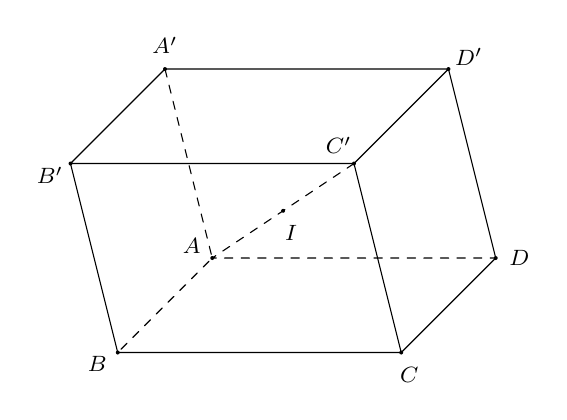
\begin{tikzpicture}[scale=.6, font=\footnotesize, line join=round, line cap=round, >=stealth]
				\path (0,0) coordinate (B) (2,2) coordinate (A) (8,2) coordinate (D) (6,0) coordinate (C) (-1,4) coordinate (B') (1,6) coordinate (A') (7,6) coordinate (D') (5,4) coordinate (C') (3.5,3) coordinate (I);
				\draw[dashed] (A')--(A)--(B) (C')--(A)--(D);
				\draw (A')--(B')--(C')--(D')--cycle
				(B')--(B)--(C)--(C') (C)--(D)--(D');
				\foreach \x/\y in {A/150,B/210,C/-70,D/0,A'/90,B'/210,C'/130,D'/30,I/-70}{\fill (\x)node[shift={(\y:3mm)}]{$\x$} circle (1.2pt);}
			\end{tikzpicture}
		\end{center}
		Tâm $I$ của hình hộp $ABCD.A'B'C'D'$ là giao điểm bốn đường chéo $AC'$, $A'C$, $BD'$ và $B'D$.\\
		Khi đó, $I$ là trung điểm của $AC'$ nên $I\left(\dfrac{5}{2};\dfrac{5}{2};-2\right)$.
	}
\end{ex}
\begin{ex}%[2H2V2-3]
	Trong không gian $Oxyz$, cho hình bình hành $ABCD$. Biết $A(1;3;2)$, $B(2;0;-2)$, $D(-3;7;1)$, và $G(a;b;c)$ là trọng tâm $\triangle BCD$. Tìm $a+3b-3c$.
	\loigiai{Ta có $\overrightarrow{AB}=(1;-3;-4)$, $\overrightarrow{AD}=(-4;4;-1)$.\\
		Gọi $C(x;y;z)$ là điểm cần tìm. Suy ra $\overrightarrow{DC}=(x+3;y-7;z-1)$.\\
		Vì $ABCD$ là hình bình hành nên $\overrightarrow{AB}=\overrightarrow{DC}$
		$\Leftrightarrow
		\heva{&x+3=1\\&y-7=-3 \\&z-1=-4}\Leftrightarrow\heva{&x=-2\\&y=4 \\&z=-3.}$\\
		Suy ra $C(-2;4;-3)$.\\
		Vì $G(a;b;c)$ là trọng tâm $\triangle BCD$ nên $\heva{&a=\dfrac{2-2-3}{3}=-1\\&b=\dfrac{0+4+7}{3}=\dfrac{11}{3}\\&c=\dfrac{-2-3+1}{3}=-\dfrac{4}{3}.}$\\
		Do đó $a+3b-3c=-1+11+4=14$.
	}
\end{ex}

\begin{ex}%[2H2V2-2]
	Trong không gian $Oxyz$, cho ba điểm $A(1;-1;1)$, $B(3;1;2)$ và $C(-1;0;3)$. Tìm tọa độ điểm $D$ sao cho tứ giác $ABCD$ là hình thang có $2$ cạnh đáy $AB$, $CD$ và có góc tại $D$ bằng $45^\circ$.
	\loigiai{
		\begin{center}
			\begin{tikzpicture}[font=\footnotesize, line join=round, line cap=round, >=stealth, scale=1]
				\path (0,0) coordinate(D)
				(5,0) coordinate(C)
				(45:2.5) coordinate(A)
				($(A)+0.55*(C)-0.55*(D)$)	coordinate(B);
				\draw (A)--(B)--(C)--(D)--cycle;
				\foreach \i/\j in {A/90, B/90, C/-90, D/-90} \fill (\i) node[shift={(\j:3mm)}]{$\i$} circle(1pt);
			\end{tikzpicture}
		\end{center}
		Đặt $D(a;b;c)$ khi đó $\overrightarrow{AB}=(2;2;1)$, $\overrightarrow{DC}=(-1-a;-b;3-c)$, $\overrightarrow{DA}=(1-a;-1-b;1-c)$.\\
		Tứ giác $ABCD$ là hình thang nên $\overrightarrow{AB}$ và $\overrightarrow{DC}$ cùng hướng hay
		\[\dfrac{-1-a}{2} = \dfrac{-b}{2} = \dfrac{3-c}{1} >0 \Leftrightarrow \heva{&a=2c-7 \\ &b=2c-6 \\ &c<3.}\]
		Khi đó $\overrightarrow{DA}=(8-2c; 5-2c; 1-c)$.\\
		Do hình thang $ABCD$ có góc tại $D$ bằng $45^{\circ}$ nên
		\begin{eqnarray*}
			&\dfrac{\sqrt{2}}{2} = \cos45^{\circ} &= \cos\left(\overrightarrow{DC}; \overrightarrow{DA}\right)=\cos\left(\overrightarrow{AB}; \overrightarrow{DA}\right) \\
			&& = \dfrac{2(8-2c)+2(5-2c)+(1-c)}{3 \cdot \sqrt{(8-2c)^2+(5-2c)^2+(1-c)^2}} = \dfrac{9(3-c)}{9\sqrt{c^2-6c+10}}\\
			&&=\dfrac{3-c}{\sqrt{c^2-6c+10}}.
		\end{eqnarray*}
		Suy ra
		\begin{eqnarray*}
			&&2(3-c)=\sqrt{2} \sqrt{c^2-6c+10}\\
			&\Rightarrow & 4(c^2-6x+9)=2(c^2-6c+10)\\
			& \Rightarrow & 2c^2-12c+16=0 \Rightarrow \hoac{&c=4 \text{ (loại, do $c<3$)}\\ &c=2 \text{ (thỏa mãn)}.}
		\end{eqnarray*}
		Với $c=2$, ta có $a=-3$ và $b=-4$. Suy ra $D(-3;-4;2)$.
	}
\end{ex}





\Closesolutionfile{ans}

